\documentclass[12pt,a4paper]{article}
\usepackage[utf8]{inputenc}
\usepackage[spanish]{babel}
\usepackage{amsmath}
\usepackage{amsfonts}
\usepackage{amssymb}
\usepackage{makeidx}
\usepackage{graphicx}
\usepackage{lmodern}
\usepackage{kpfonts}
\usepackage{apacite}
\usepackage{multirow}
\usepackage{multirow}
\usepackage{graphicx}
\setlength{\parindent}{0em}
\usepackage[left=3cm,right=3cm,top=2cm,bottom=2cm]{geometry}
\author{Pablo Vivas Corrales\footnote{\textit{Maestría Académica en Estadística. Universidad de Costa Rica}}\\\textit{pablo.vivas@ucr.ac.cr}}
\title{Análisis espacial del dengue en Costa Rica}
\date{16 de diciembre de 2019}
\begin{document}
\maketitle
\begin{abstract}
\noindent
La posición geográfica de Costa Rica posibilita al vector \textit{Aedes} la propagación de la enfermedad conocida como dengue. Solo en el año 2019 la sección de vigilancia del Ministerio de Salud reportó más de 8000 mil casos de esta enfermedad. Con esos datos e información obtenida del Instituo Nacional de Estadistica y Censos (INEC) se realizó un análisis espacial con los siguientes objetivos: \\
\textbf{Palabras clave:} \textit{Palabra 1, Palabra 2, Palabra 3 \& Palabra 4} 
\end{abstract}
\section{Introducción}

El dengue es una enfermedad aguda febril, producida por un virus ARN de la familia \textit{Flaviridae}, cuyo único reservorio es el hombre. Existen 4 serotipos distintos DEN- 1, DEN- 2, DEN- 3 y DEN- 4. Es más predominante en las regiones tropicales. El virus se transmite por la picadura de la hembra del mosquito \textit{Aedes sp.} Ésta adquiere la infección al alimentarse de un paciente en fase virémica. El virus se multiplica y alcanza las glándulas salivares de la mosquito hembra, donde se mantiene de por vida, por lo que puede infectar a varias personas. Existen varios tipos de Aedes: Ae. aegypti, Ae. albopictus, Ae. meiovittatus, Ae. scutellaris .etc. El más importante es Ae. aegypti, que se alimenta principalmente sangre humana y lo hace de día. El virus es altamente transmisible cuando la infestación por el vector es alta, lo que puede producir epidemias de dengue con alta morbilidad y mortalidad, en su forma grave. La infección que produce resulta en un amplio espectro de presentaciones clínicas, que van desde formas asintomáticas, indiferenciadas y leves hasta cuadros graves con compromiso vascular, coagulación y órganos blancos.Puede haber transmisión por la picadura directa del mosquito, vía vertical (madre-hijo,tercer trimestre de embarazo) o vía transfusional \cite{CajaCostarricensedelSeguroSocial2013}.
\section{Métodos}

Los datos utilizados utilizados para realizar el análisis espacial del dengue en Costa Rica provienen de dos fuentes. En primer lugar, de la sección de vigilancia del Ministerio de Salud se obtiene la información de los casos de dengue para el 2019 por cantón. Los paquetes de R \cite{R} de readxl \cite{readxl}, sp \cite{sp}, sf \cite{sf}, tidyverse \cite{tidy}, rgdal \cite{rdal}, RColorBrewer \cite{Rcolor}, spdep \cite{sp}, tmap \cite{tmap}, tmaptools \cite{tmaptools}, spatialreg \cite{sp}, epitools \cite{epitools}, DCluster \cite{dcluster}, plotrix \cite{plotrix}, MASS \cite{MASS} \& mgcv \cite{mgcv}.
\section{Resultados}

\begin{figure}[hbtp]
\centering
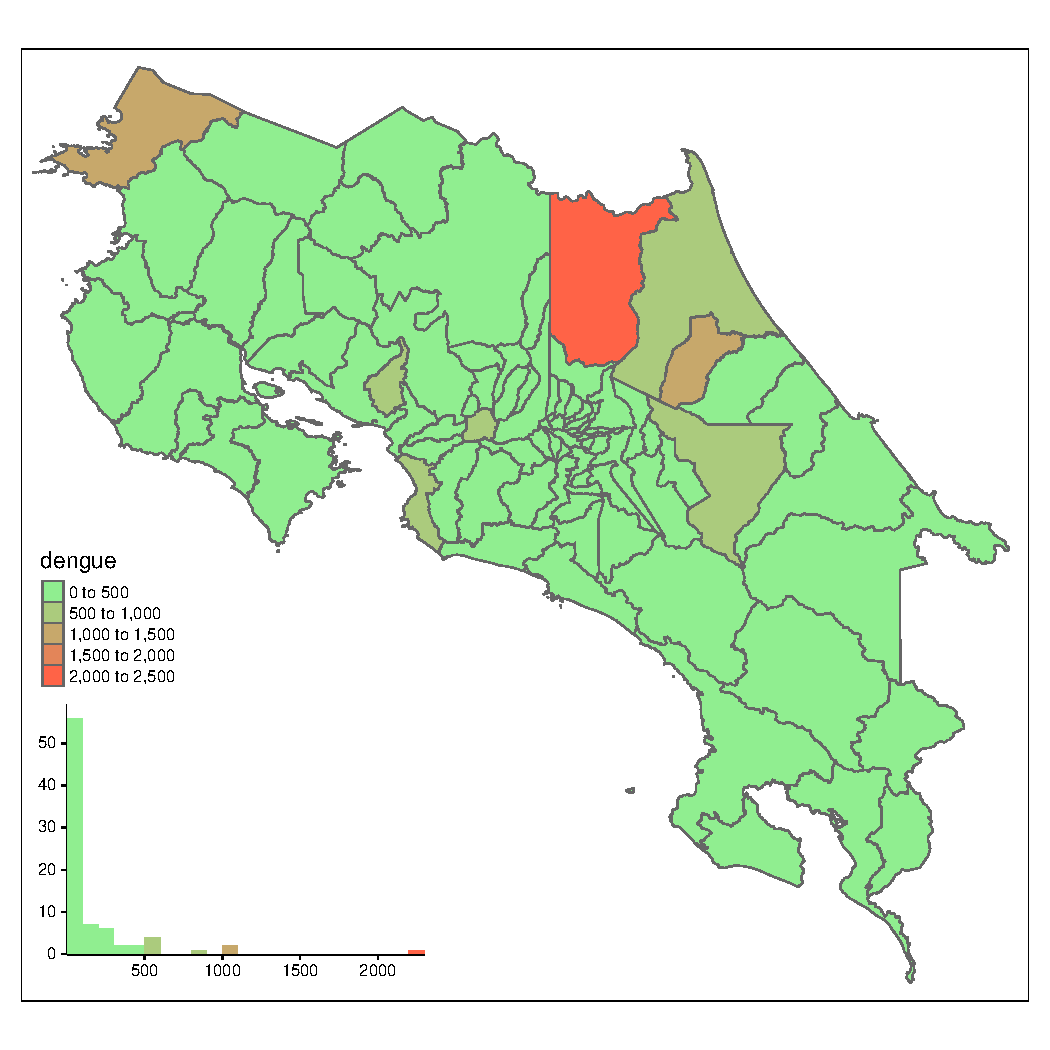
\includegraphics[width=.48\textwidth]{F11.pdf}
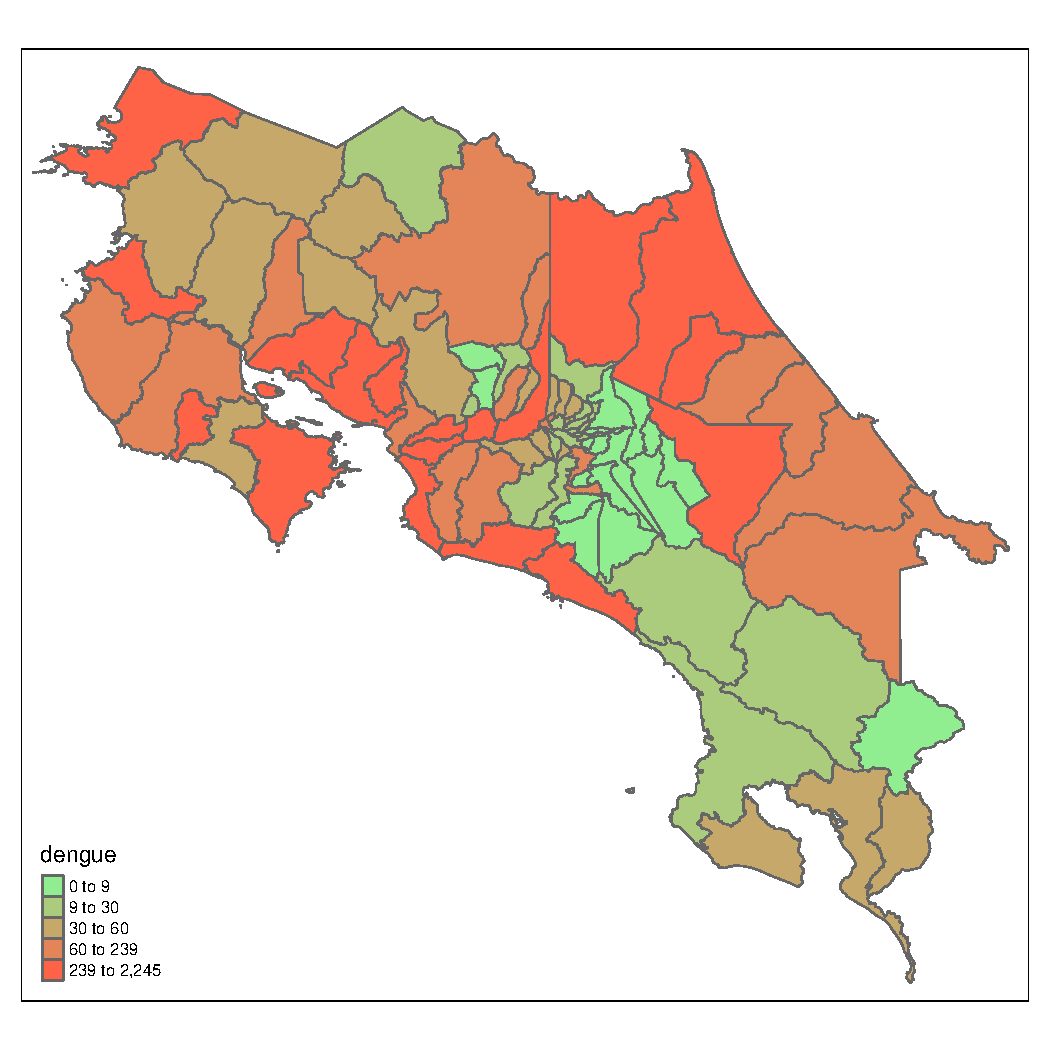
\includegraphics[width=.48\textwidth]{F12.pdf}
\caption{Tasa de dengue (100.000 habitantes) por cantón, 2019.}
\end{figure}

\begin{figure}[hbtp]
\centering
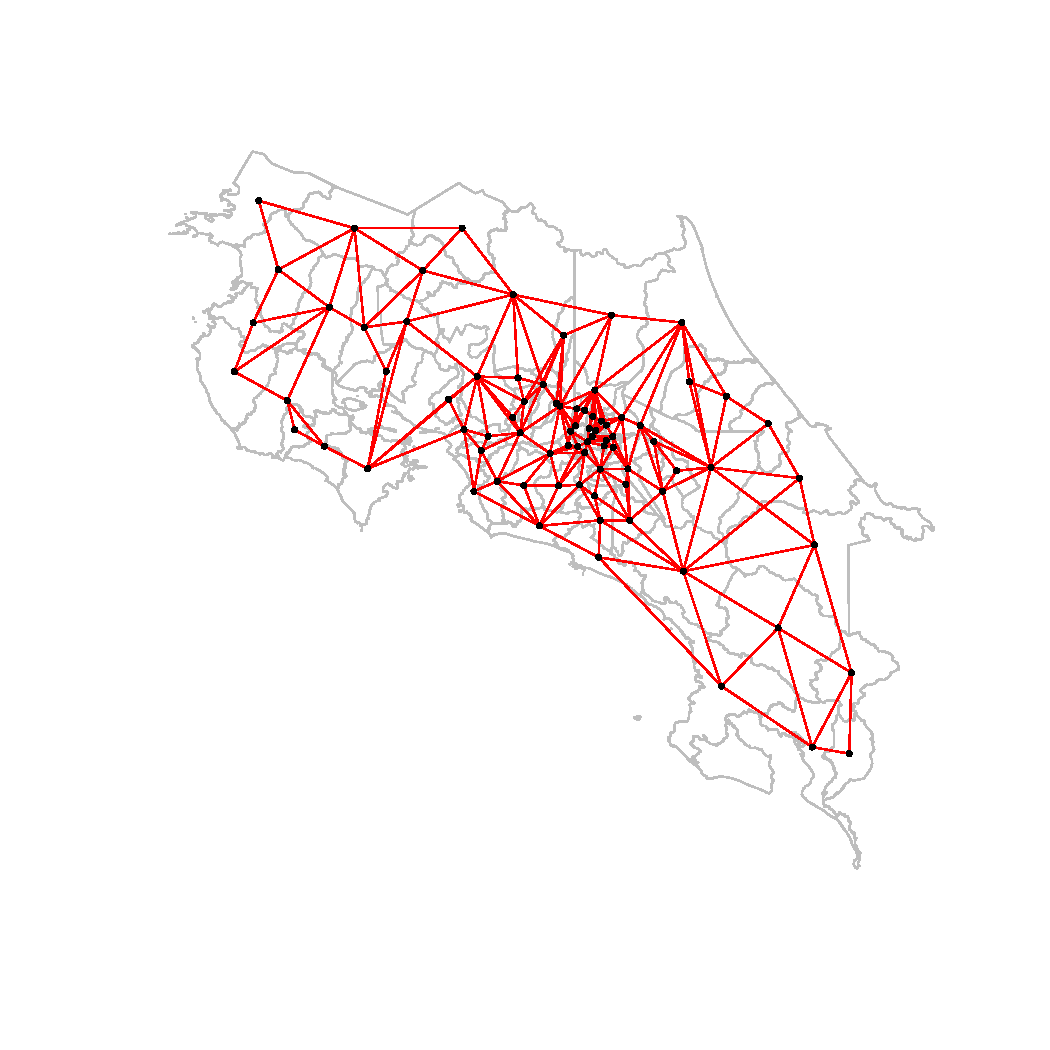
\includegraphics[width=.48\textwidth]{F21.pdf}
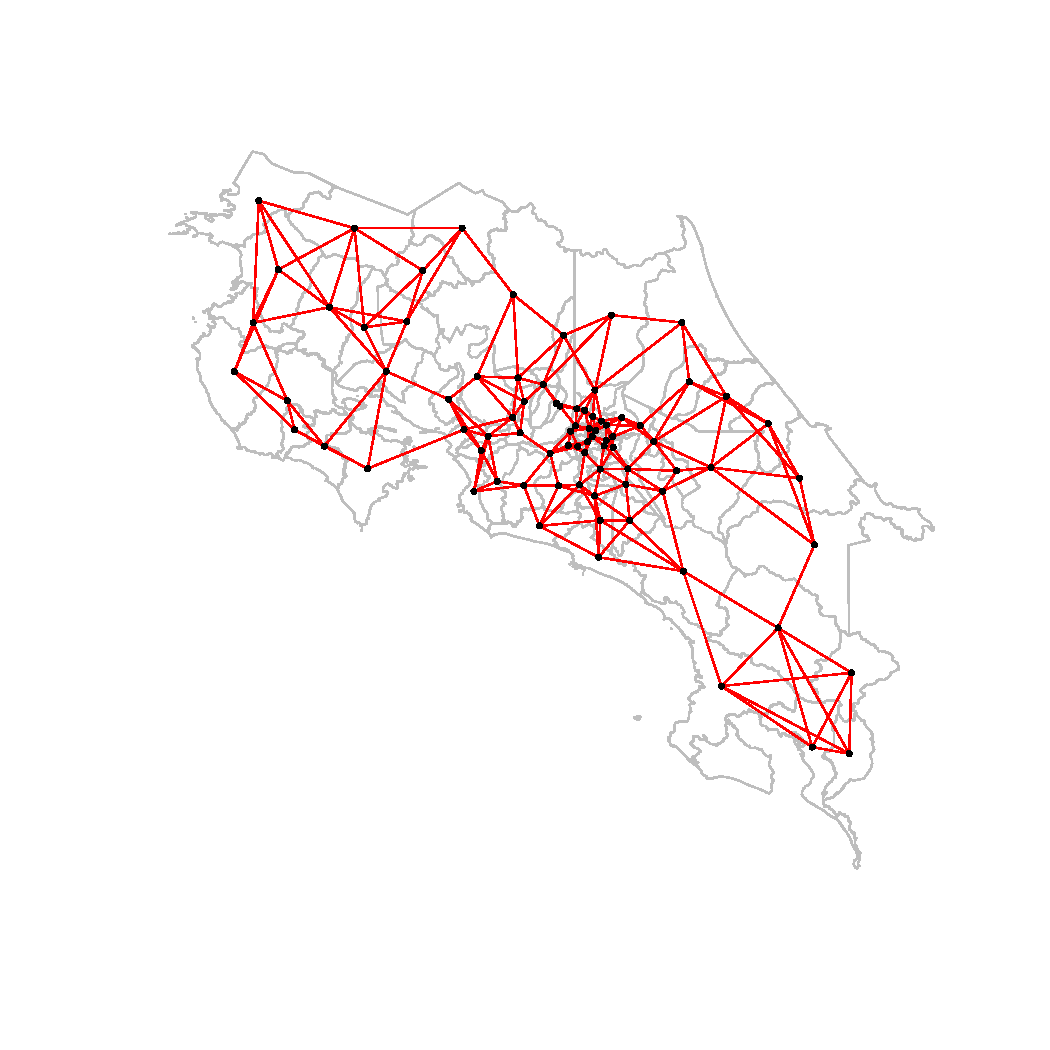
\includegraphics[width=.48\textwidth]{F22.pdf}
\caption{Métodos de vecinos: Reina y Knn(4)}
\end{figure}

\begin{figure}[hbtp]
\centering
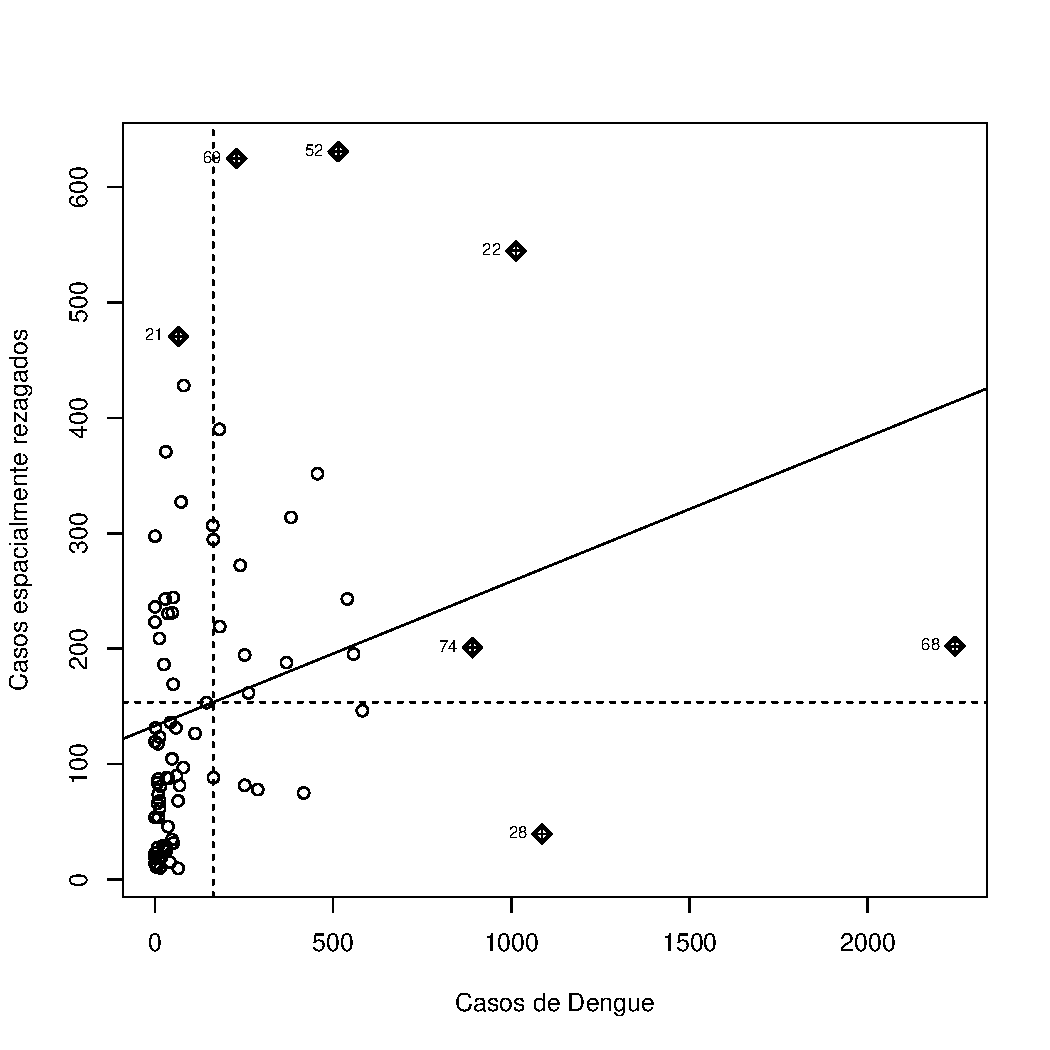
\includegraphics[width=.48\textwidth]{F31.pdf}
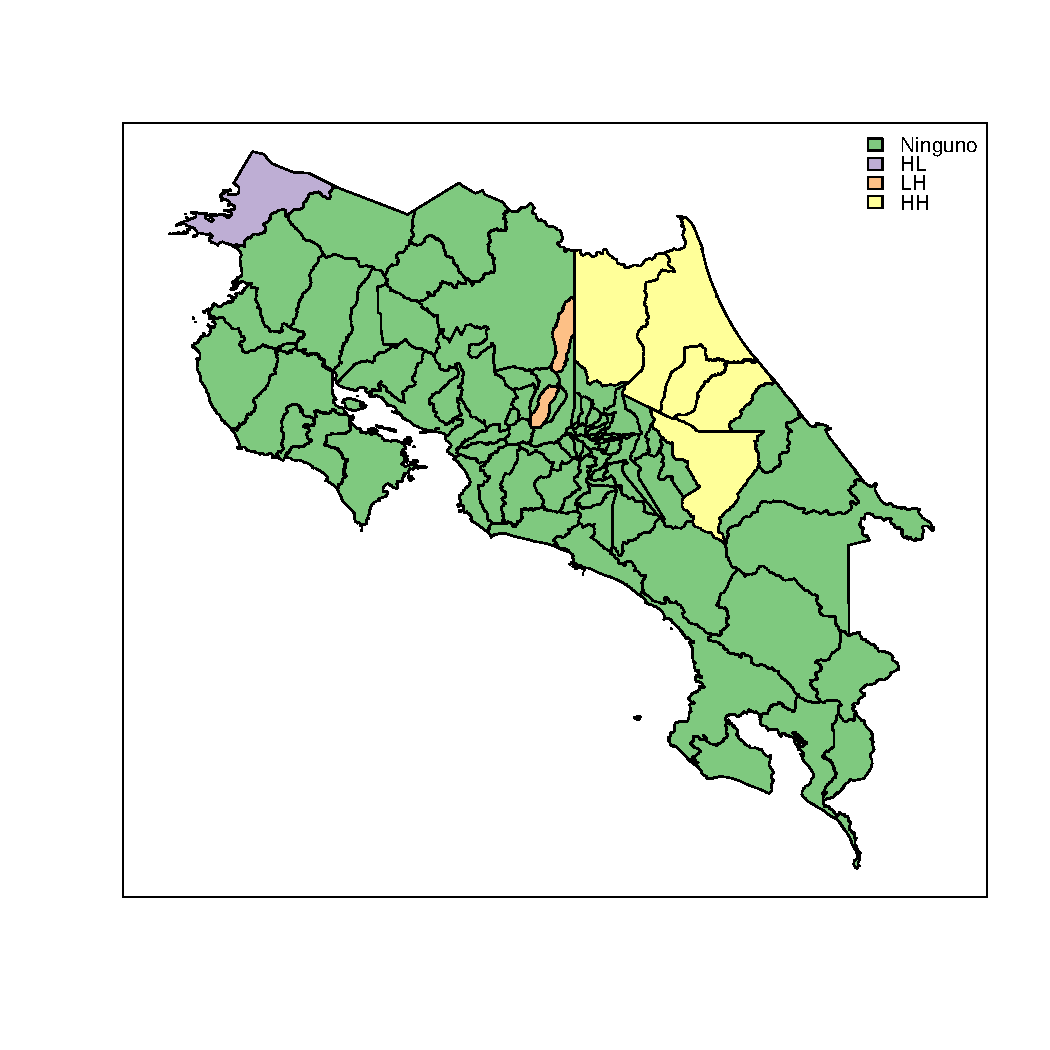
\includegraphics[width=.48\textwidth]{F32.pdf}
\caption{Casos de influencia}
\end{figure}

\begin{figure}[hbtp]
\centering
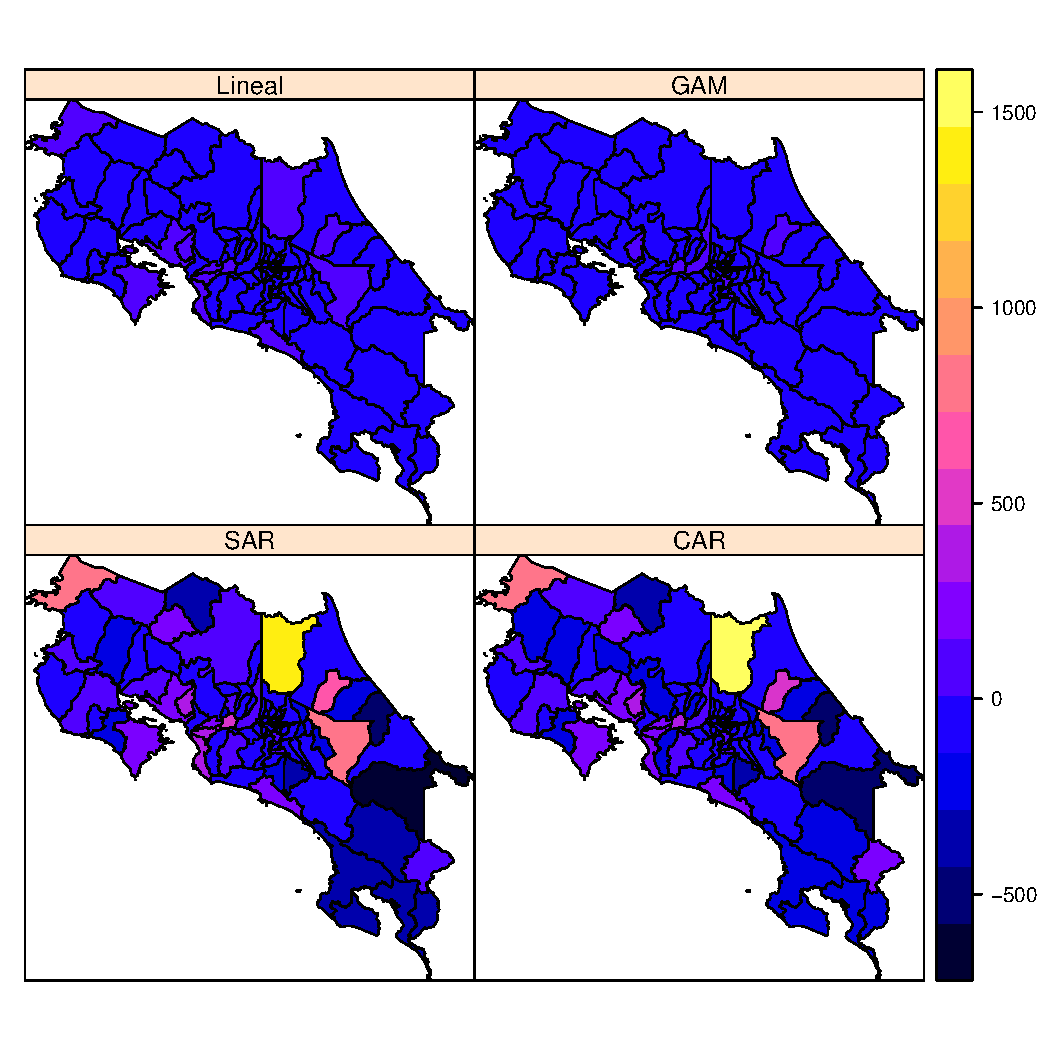
\includegraphics[scale=0.75]{F4.pdf}
\caption{Residuales de los modelos}
\end{figure}

\begin{figure}[hbtp]
\centering
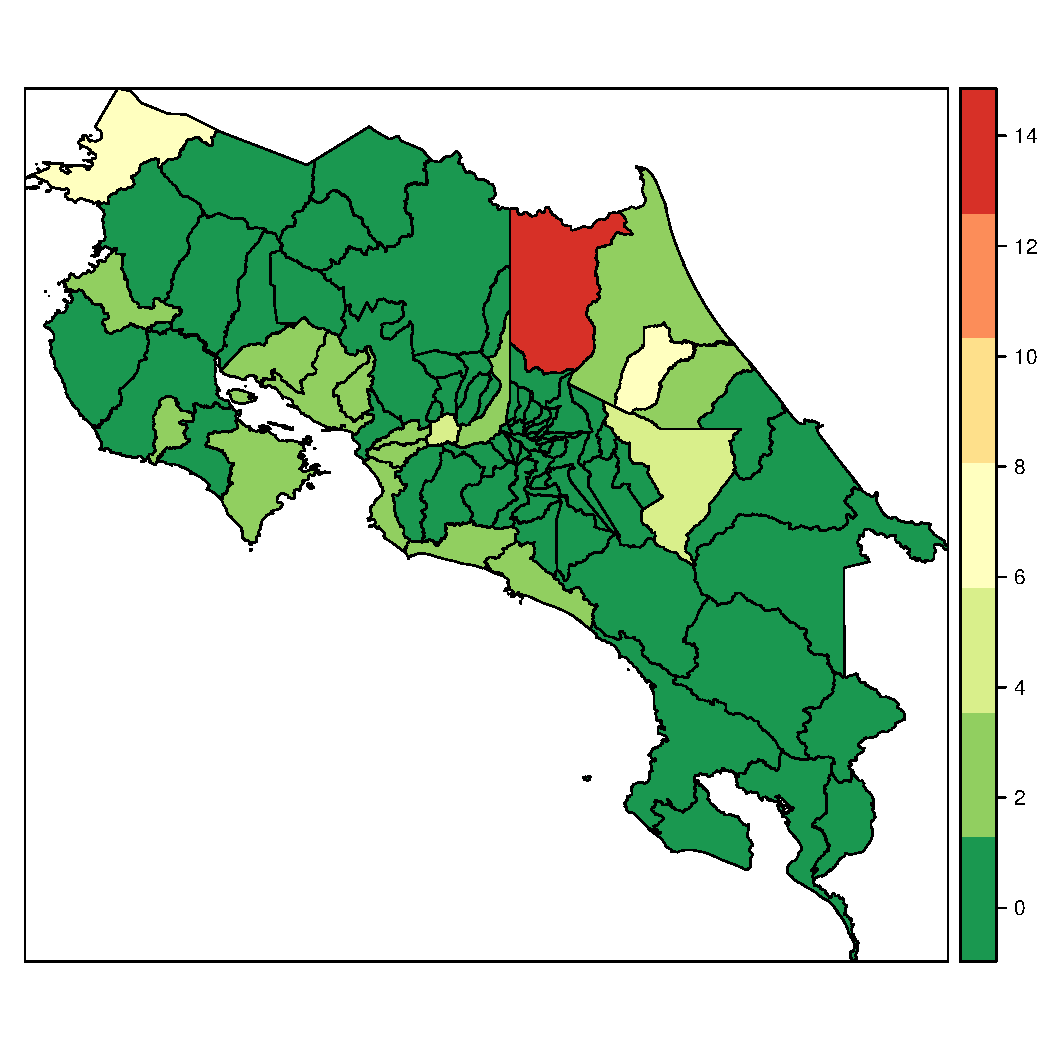
\includegraphics[scale=0.5]{F5.pdf}
\caption{Riesgo relativo}
\end{figure}

\begin{figure}[hbtp]
\centering
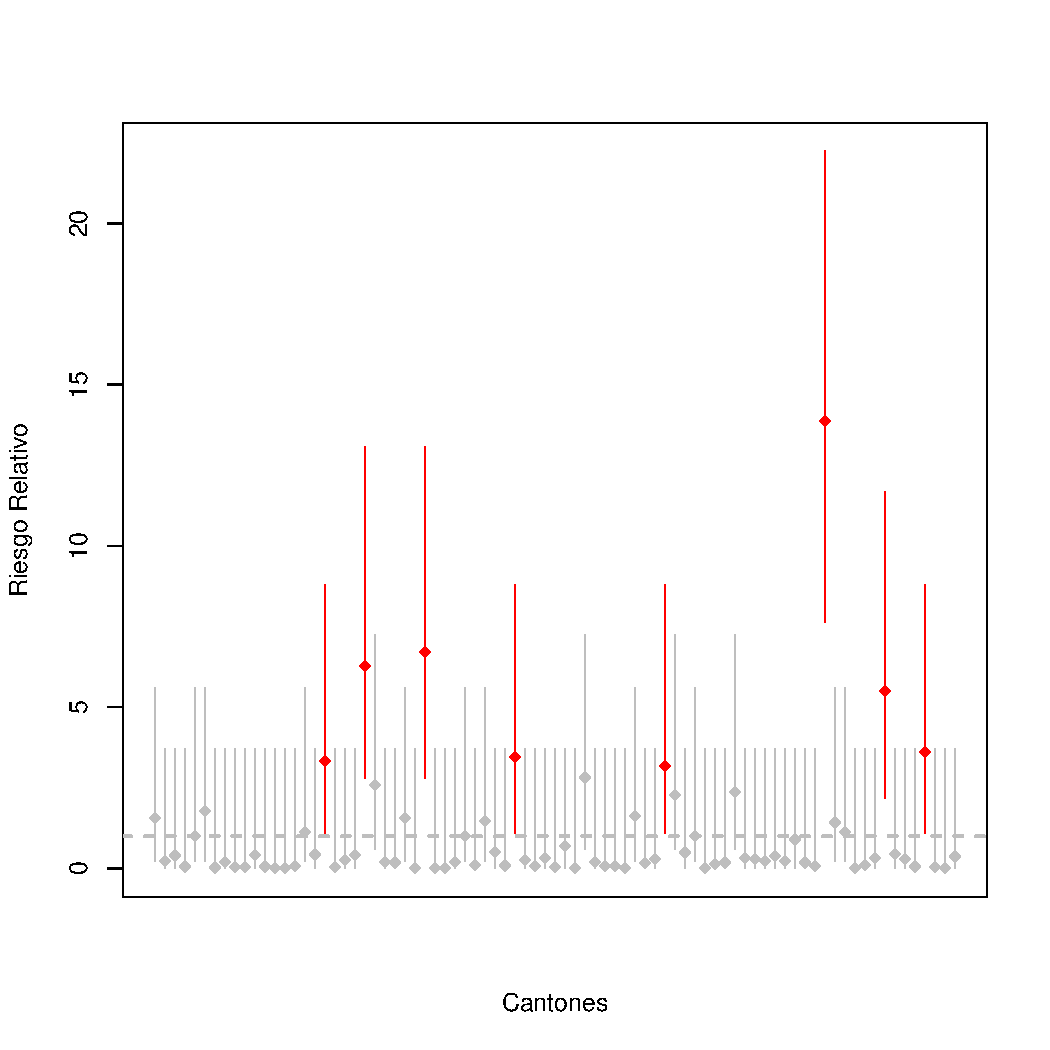
\includegraphics[scale=0.75]{F6.pdf}
\caption{Intervalos de confianza}
\end{figure}

\begin{table}[h]
\centering
\begin{tabular}{cccc}
\hline
\multirow{2}{*}{Vecinos} & \multicolumn{3}{l}{Matriz de pesos}\\ \cline{2-4} 
&W&B&S\\ \hline
Reina&0,009&0,007&0,006\\
Torre&0,011&0,008&0,008\\
Knn(2)&0,018&0,018&0,018\\
Knn(4)&0,026&0,026&0,026\\ \hline
\end{tabular}
\end{table}

\section{Conclusiones}

\section{Anexos}

\begin{figure}[hbtp]
\centering
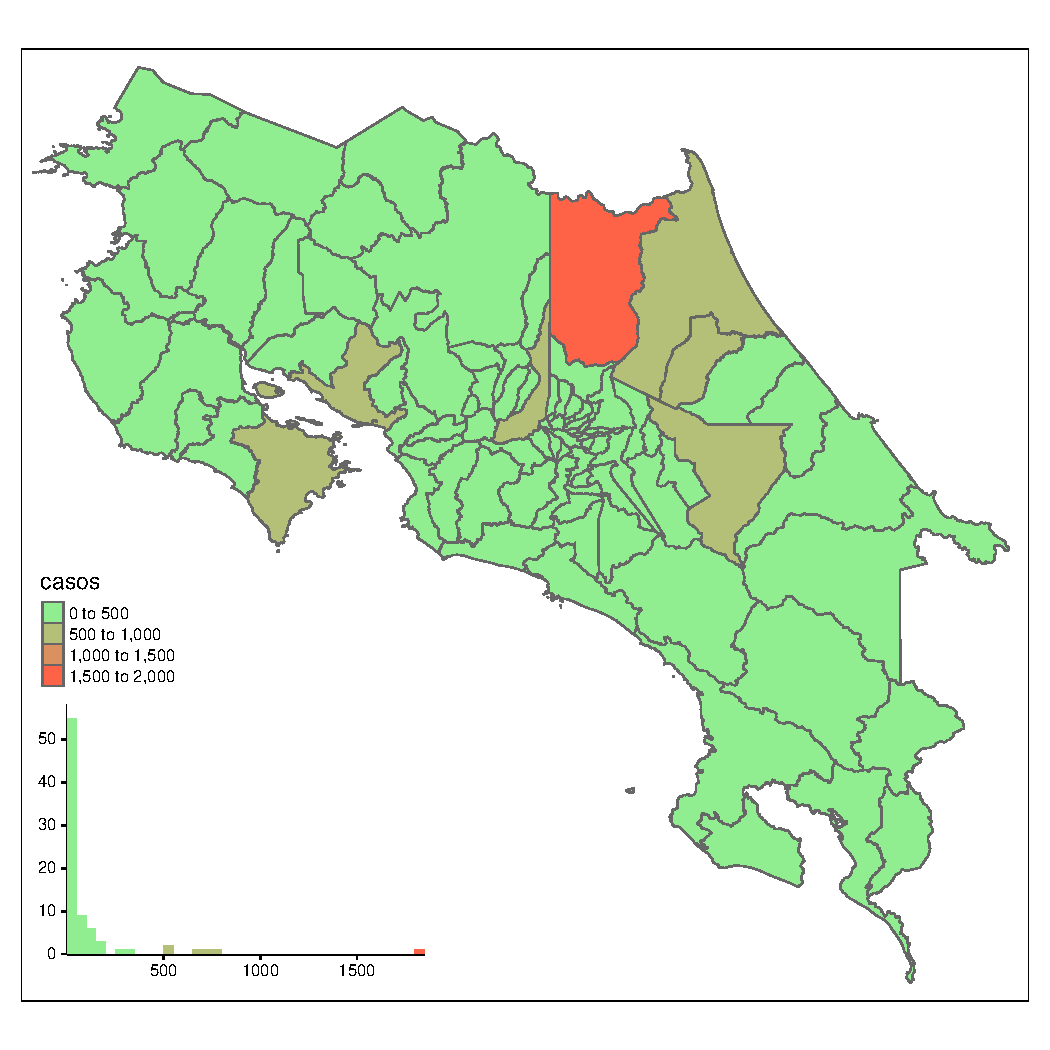
\includegraphics[width=.48\textwidth]{FA1.pdf}
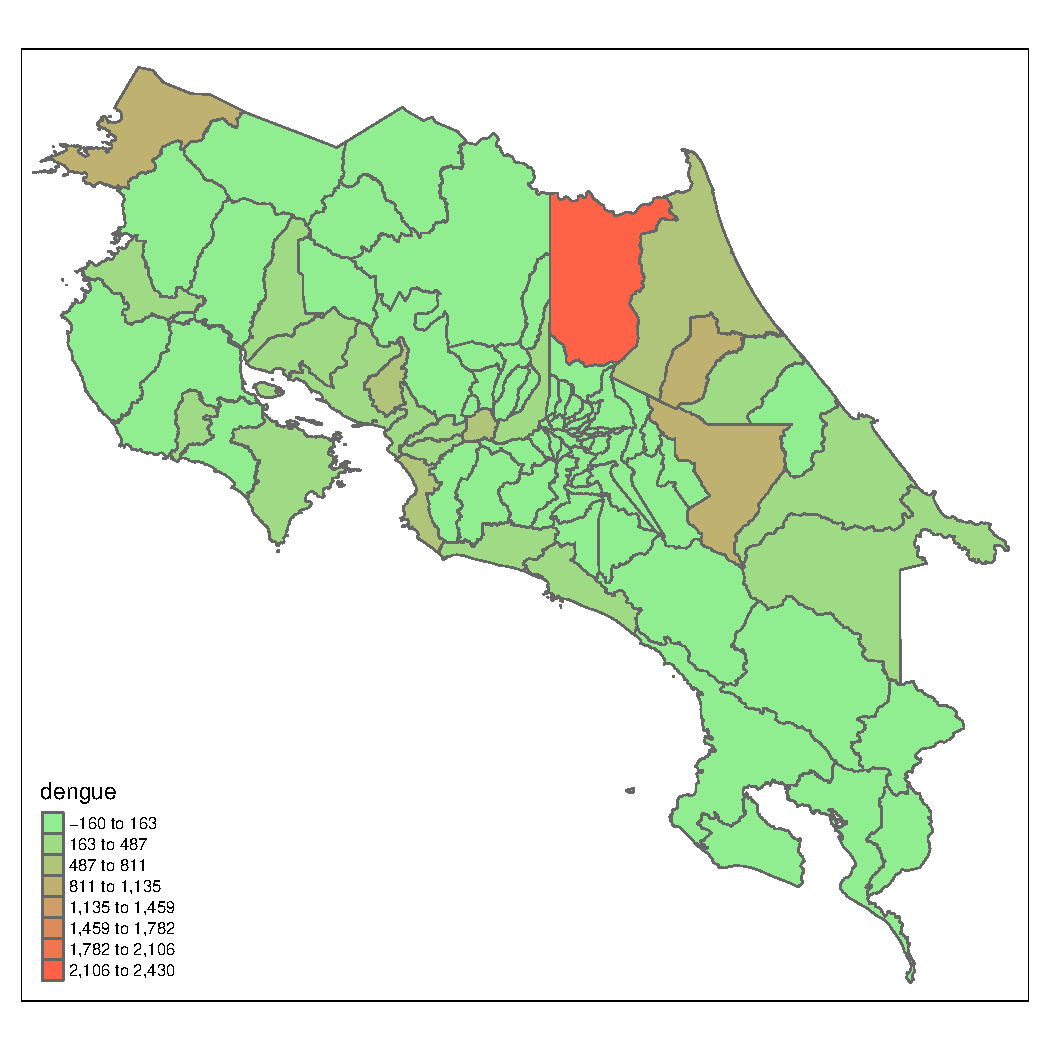
\includegraphics[width=.48\textwidth]{FA2.pdf}
\caption{Casos de dengue (100.000 habitantes) por cantón, 2019.}
\end{figure}

\begin{figure}[hbtp]
\centering
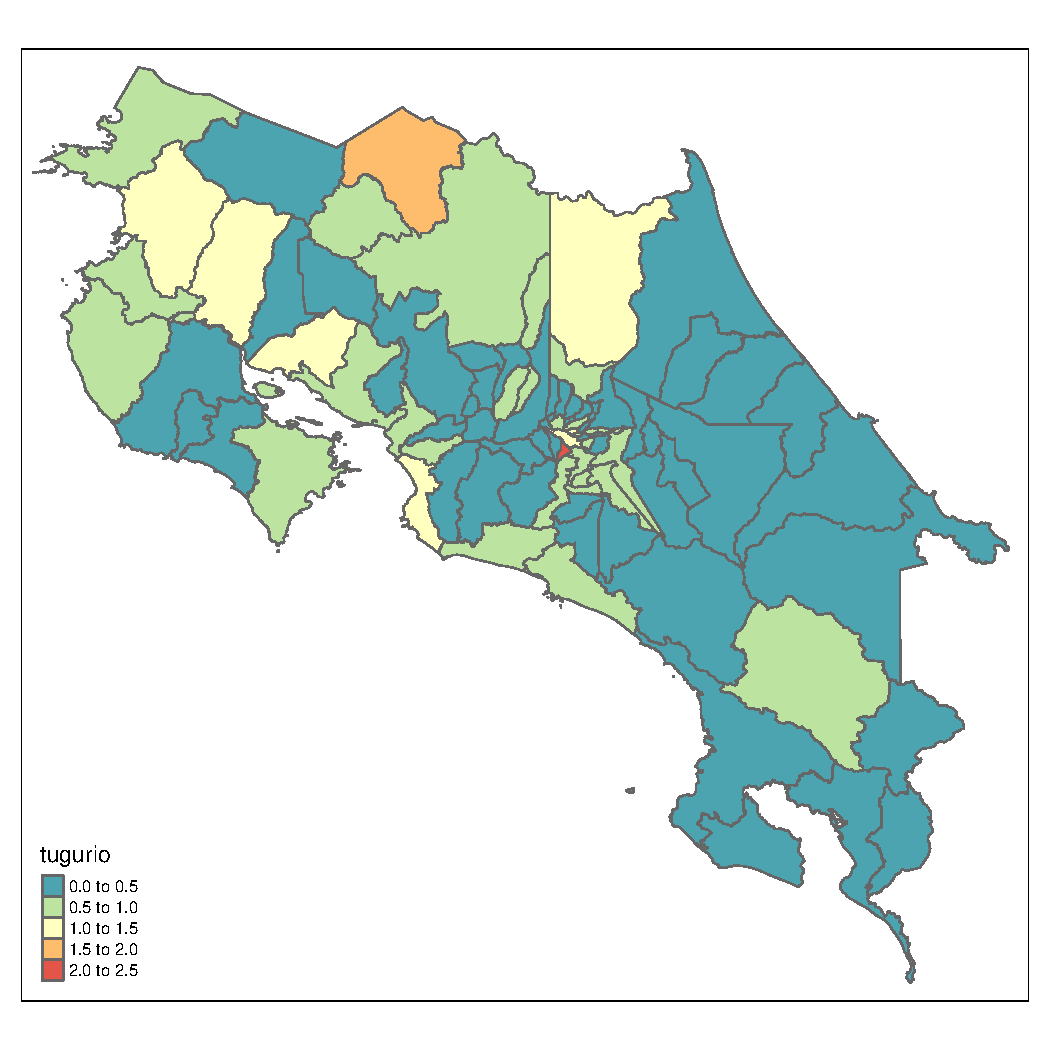
\includegraphics[width=.48\textwidth]{FA3.pdf}
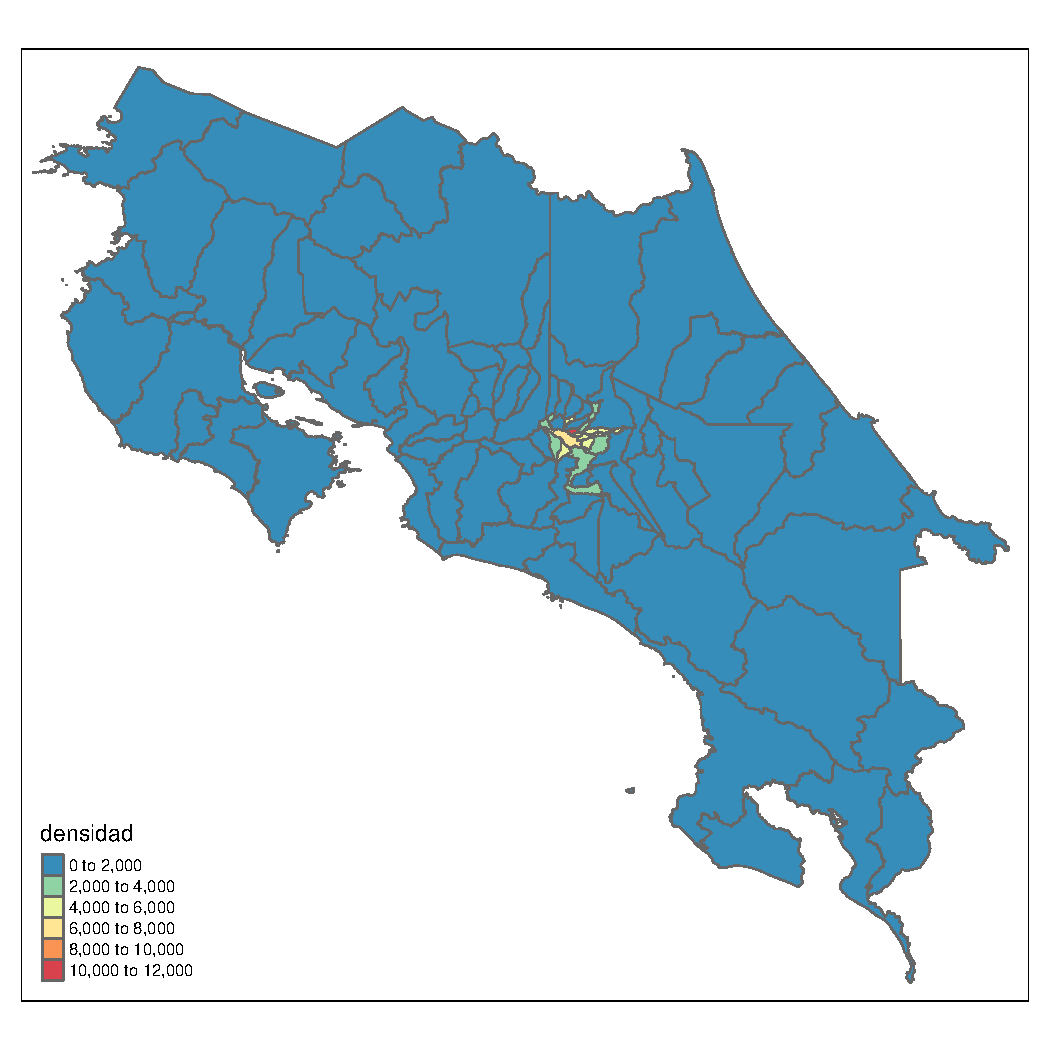
\includegraphics[width=.48\textwidth]{FA4.pdf}
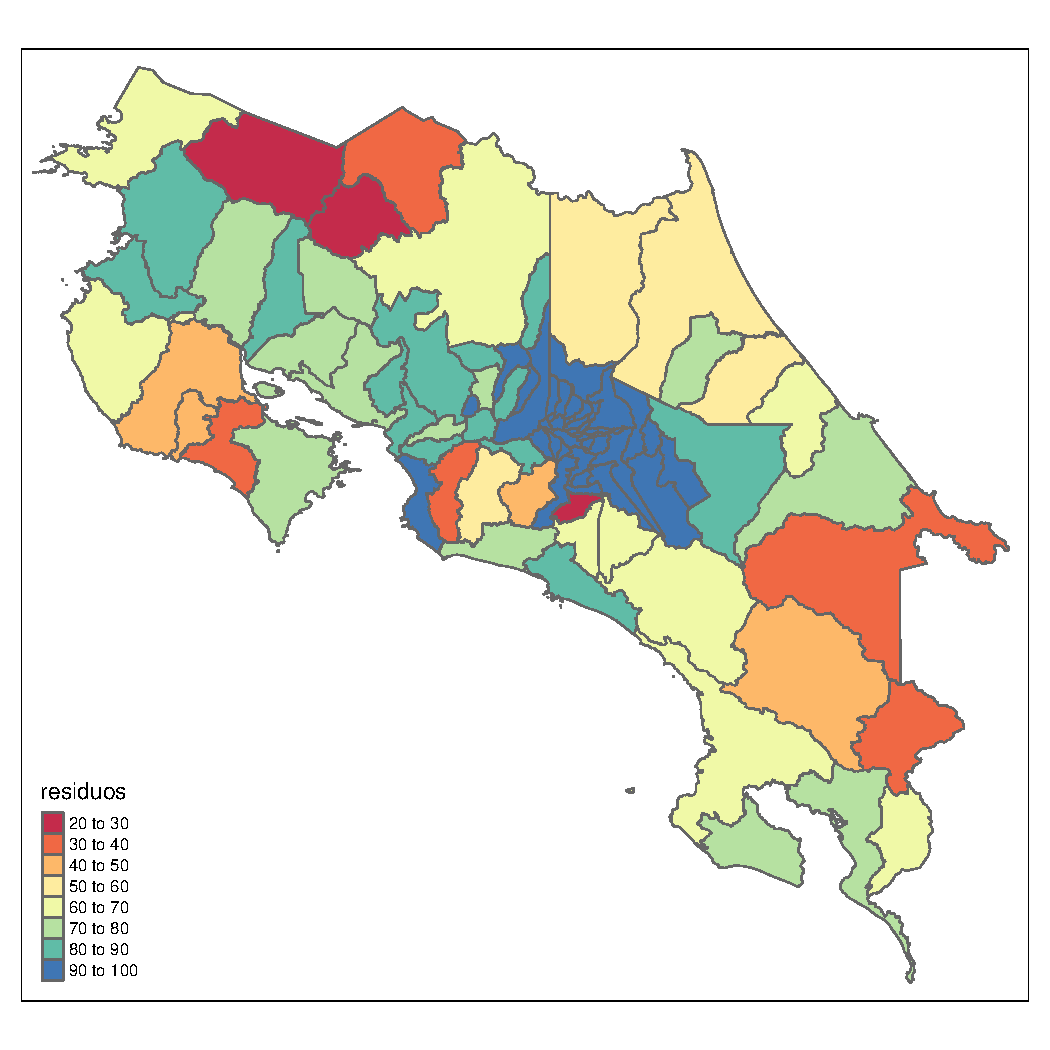
\includegraphics[width=.48\textwidth]{FA5.pdf}
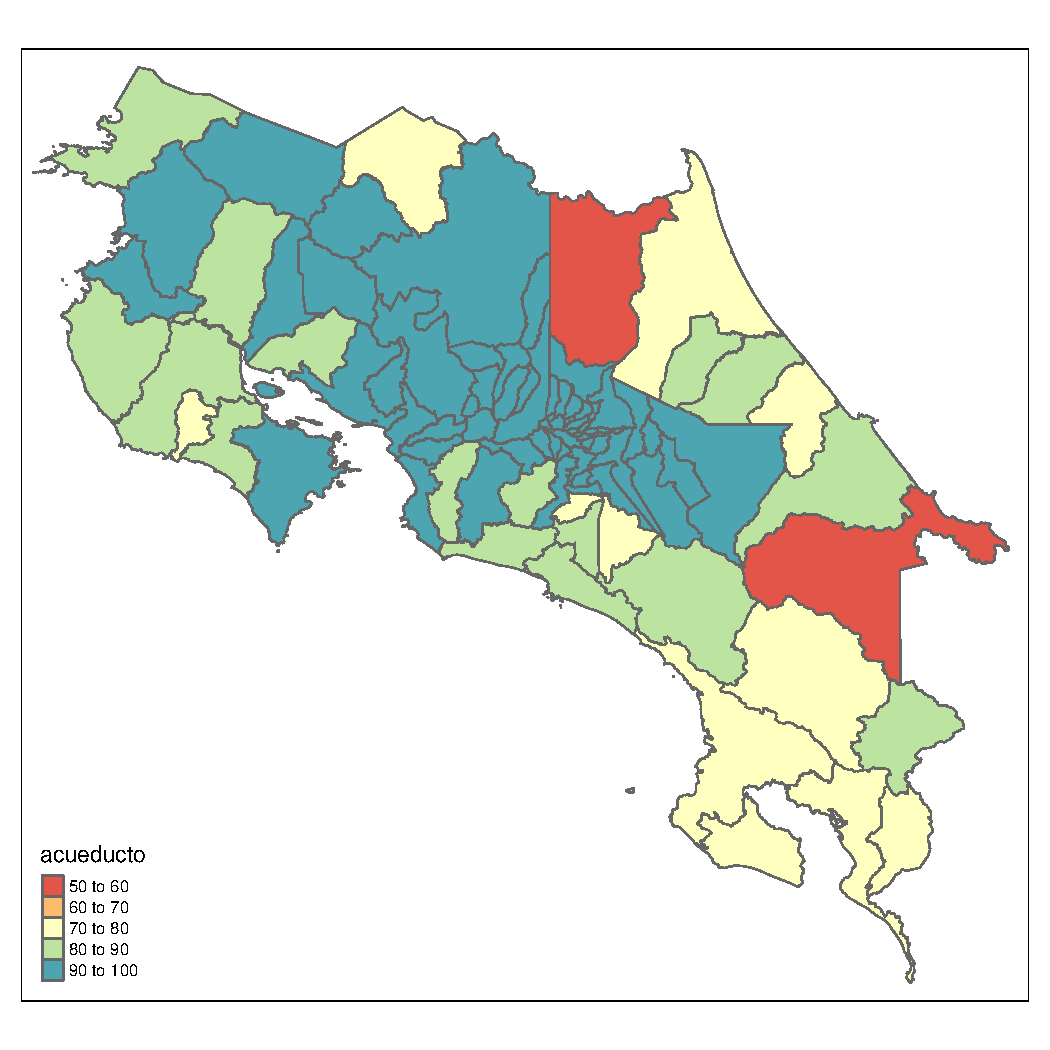
\includegraphics[width=.48\textwidth]{FA6.pdf}
\caption{Estadísticos descriptivos}
\end{figure}

\begin{figure}[hbtp]
\centering
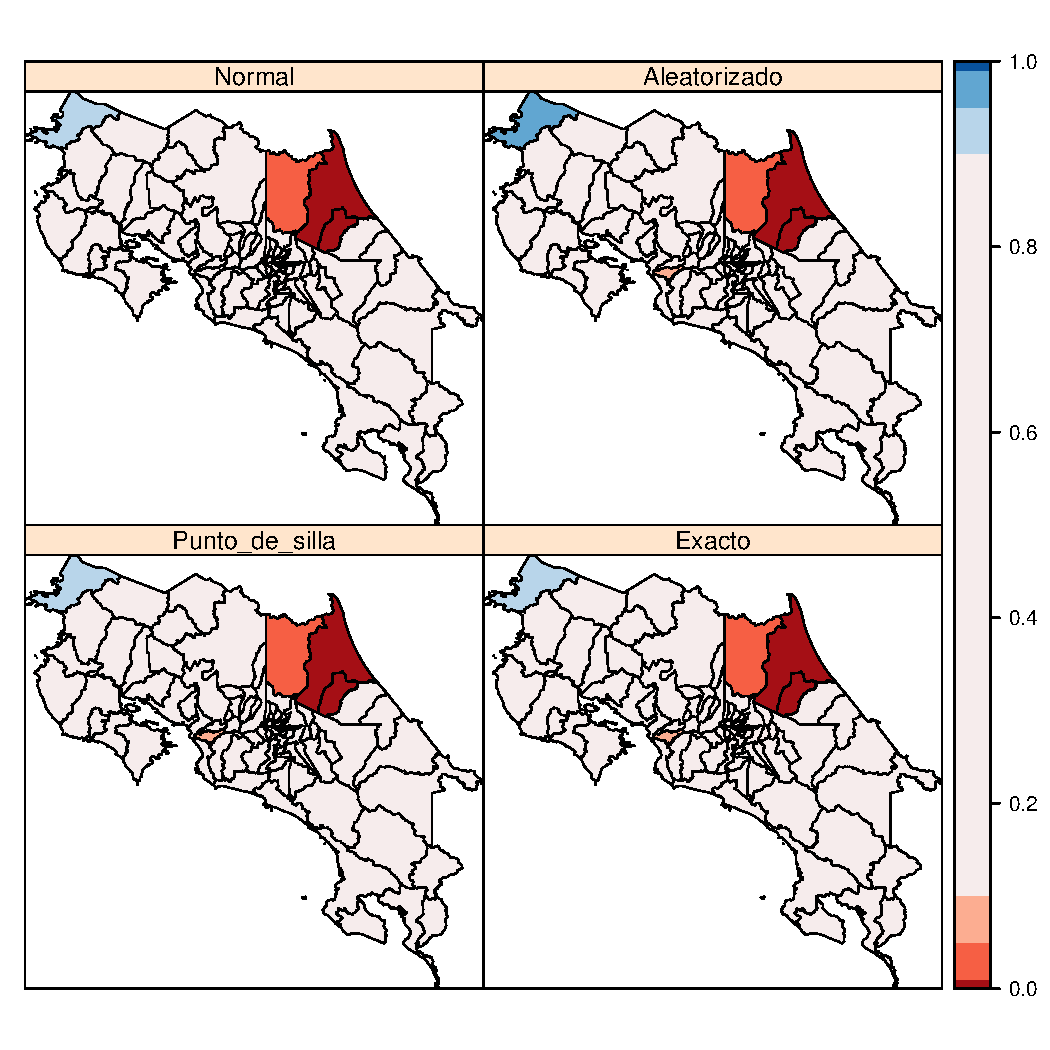
\includegraphics[scale=0.75]{FA7.pdf}
\caption{Distintas pruebas de Moran}
\end{figure}

\begin{figure}[hbtp]
\centering
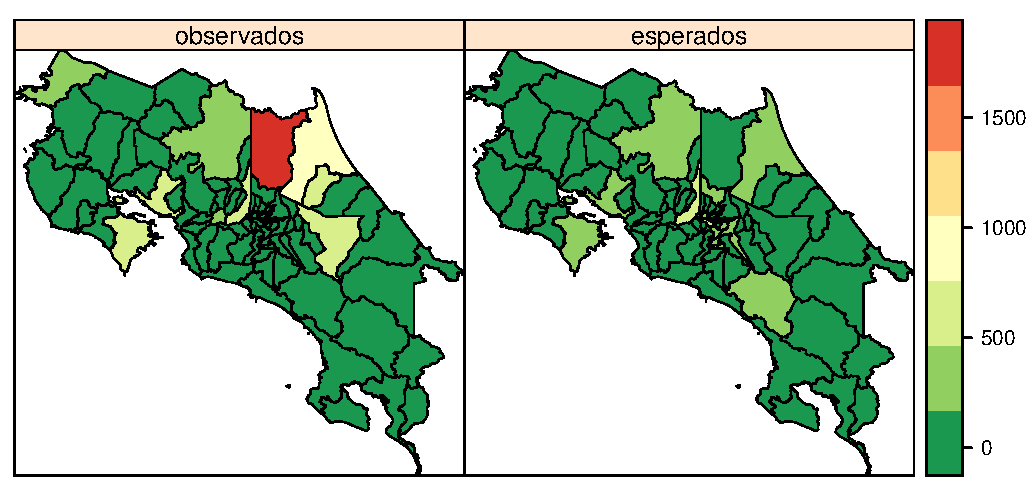
\includegraphics[scale=0.75]{FA8.pdf}
\caption{Valores Observados vs Esperados}
\end{figure}

\begin{figure}[hbtp]
\centering
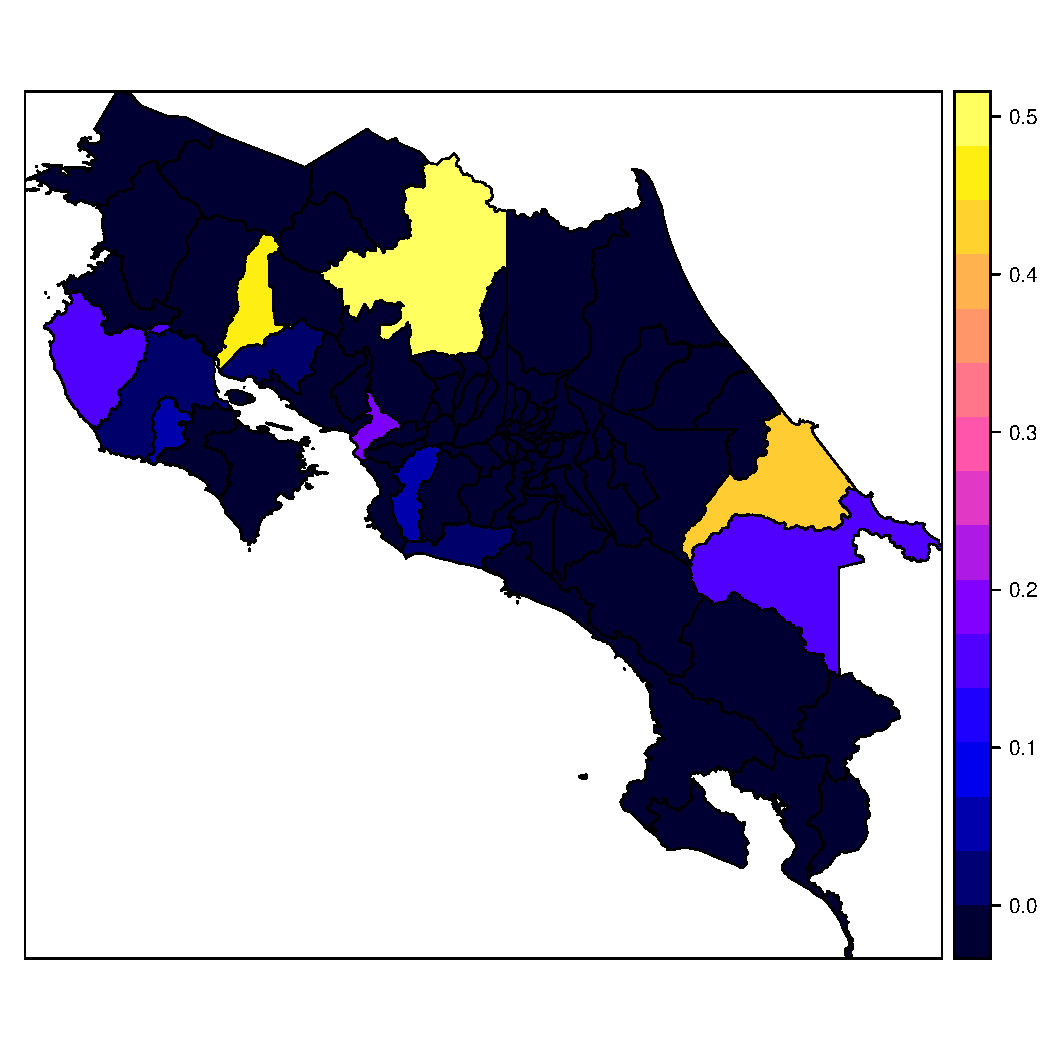
\includegraphics[scale=0.75]{FA9.pdf}
\caption{Mapa de probabilidad de Chownoysky}
\end{figure}

\begin{figure}[hbtp]
\centering
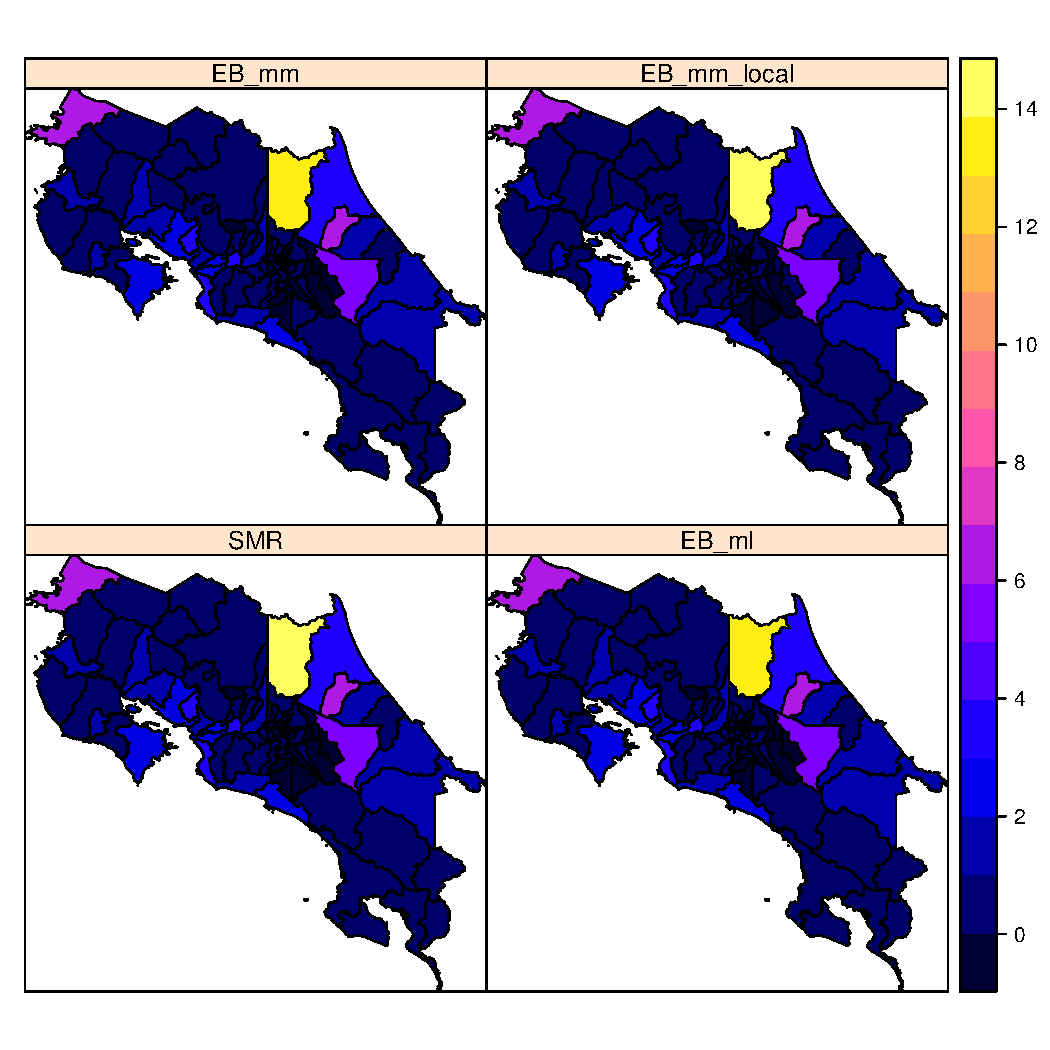
\includegraphics[scale=0.75]{FA10.pdf}
\caption{Distintas pruebas de Moran}
\end{figure}

%%Bibliografía
\bibliographystyle{apacite}
\bibliography{Referencias}
\end{document}


